\section{Ecossistema de software acadêmico de análise estática} \label{analise-estatica}

Ao falarmos sobre ecossistema de software acadêmico estamos nos referindo a
qualquer software, de qualquer domínio de aplicação, que tenha sido utilizado
ou produzido durante trabalhos de pesquisa com intuito de publicação na
literatura acadêmica.
%REVER - intuito de apoiar pesquisa que será eventualmente divulgada por meio da  publicação de resultados.

O ecossistema de software acadêmico de análise estática é um recorte deste
conjunto, a princípio, com as mesmas características, atores e modelo de
funcionamento, mas logicamente podendo de apresentar particularidades trazidas
pela natureza do domínio de análise estática e suas ferramentas, soluções e
algoritmos.

\subsection{Análise estática}

A análise estática de código fonte é o primeiro passo para coletar informações
necessárias em diversas atividades de verificação, medição e melhoria da
qualidade de produtos de software \cite{Cruz2009, Kirkov2010}. Ela é
realizada com base no código fonte de um programa ou sistema de software, e a
partir daí descobre problemas e propriedades de sua qualidade estrutural
\cite{Chess2007}.

Ferramentas de análise estática estão disponíveis há décadas, em especial,
para programadores. A ferramenta Lint \cite{Johnson1978}, considerada a
primeira ferramenta de análise estática \cite{Gosain2015}, foi criada para
examinar programas escritos em linguagem C e aplicar regras de tipagem mais
estritas do que as regras dos próprios compiladores da linguagem.

Análise estática de código fonte tem como objetivo prover
informações acerca de um programa a partir do seu código fonte sem
necessidade de execução, e sem requerer qualquer outro artefato do programa
além do próprio código.

É um ramo que possui muitas das suas abordagens em comum com os estudos da
área de análise de programas ({\it program analysis}), especialmente na área de
compiladores, onde atua especialmente nas primeiras etapas do processo de compilação.

A análise estática de código fonte é considerada uma atividade meio com
objetivo de suportar uma variedade de tarefas comuns da engenharia de
software; muitas dessas tarefas são substancialmente úteis em atividades de
manutenção. Binkley~\citeonline{Binkley2007} define uma lista dessas
atividades, incluindo:

\begin{multicols}{2}
  \begin{itemize}
    \item Análise de performance
    \item Compreensão de programas
    \item Desenvolvimento baseado em modelos
    \item Detecção de clones
    \item Evolução de software
    \item Garantia de qualidade
    \item Localizaçao de falhas
    \item Manutenção de software
    \item Recuperação arquitetural
    \item Testes
  \end{itemize}
\end{multicols}

Seja em qual atividade for, a análise estática possui importância,
pois ao ser capaz de extrair informações diretamente do
código fonte de um programa, pode auxiliar a responder perguntas necessárias
para as diversas atividades de desenvolvimento e evolução de software. Essa
importância se torna ainda mais aparente diante da ``lei'' da tendência para
execução \cite{Harman2010} que indica que todos os tipos de notação tem a
tendência de se tornar executáveis.

% \subsection{Usos da análise estática de código fonte} \label{usos}

A análise de programas trata, de modo geral, da descoberta de problemas e
fatos sobre programas. Tal análise pode ser realizada sem a necessidade de executar o
programa (análise estática) ou com informações provenientes de sua execução
(análise dinâmica).

A ideia de que programas de computador podem ser utilizados para analisar
código fonte de outros programas tem uma história de mais de 40 anos.  O
programa PFORT \cite{Ryder1974} foi projetado para localizar potenciais
problemas na portabilidade de código Fortran; em função da diversidade de
dialetos de Fortran, uma compilação sem erros não indicava que o programa
estava correto segundo os padrões da linguagem \cite{Wichmann1995}.

Desde então, ferramentas de análise estática de código fonte têm surgido para
os mais diversos fins -- muitas delas a partir das pesquisas e
desenvolvimentos da área de compiladores.  O {\it parser} utilizado nessas
ferramentas têm funcionalidades análogas aos analisadores usados em
compiladores \cite{Anderson2008}.

O uso de tais ferramentas tem se tornado mais comum no ciclo de desenvolvimento de
software, sendo aplicadas em atividades distintas.
O campo de aplicação destas ferramentas é bastante variado, cobrindo diferentes
objetivos.

\subsection{Software de análise estática}

A variedade de aplicação e a constante evolução da área de análise estática, 
tanto na indústria quando na academia, resulta em  estudos teóricos e práticos, novas ferramentas, modelos e
algoritmos de análise estática. Ferramentas de análise estática têm sido
continuamente desenvolvidas e seu uso se tornado comum no ciclo de desenvolvimento de
software.

%, faz um estudo
%propondo uma taxonomia e um conjunto de dimensões para caracterização de
%ferramentas de análise estática \cite{Novak2010}.

Mas apesar da rápida e constante evolução da área, ainda há carência de estudos
avaliando estas ferramentas \cite{Li2010}, mesmo com os avanços e com
ferramentas de sucesso, o desenvolvimento de análise estática ainda é conhecido
por ser um processo doloroso \cite{toman2017taming}.

A eficiência, confiabilidade e precisão dessas ferramentas têm sido avaliadas e
alguns estudos mostram inconsistência entre ferramentas diferentes.
Um estudo que comparou duas ferramentas de análise estática para cálculo de métricas,
revelou significantes evidências sobre a inconsistencia entre valores de métricas,
grande diferença nos valores, e discutiu quais problemas e questões levam a estas
diferenças \cite{Alemerien2013}.

Análise estática é a técnica mais amplamente utilizada para análise
automatizada de programas devido a sua eficiência, boa cobertura e automação.
Estudos mostram que analise estática tem grande adoção em projetos de software
livre \cite{beller2016analyzing}.
Entretanto,tecnicas de analise estatica amplamente adotadas na comunidade de software,
por exemplo, para localização de bugs e verificação de programas 
ainda sofrem de alto indica de falso-positivos \cite{Gosain2015}.

A crescente atenção que as técnicas de análise estática de código tem
recebido em pesquisas não necessariamente influencia em sua adoção na indústria,
identificando um gap entre pesquisa e indústria \cite{ilyas2016static}.

%e
%mostra onde pode-se melhorar no desenvolvimento dessas ferramentas para
%aumentar a adoção \cite{beller2016analyzing}.

%, informações
%limitadas a respeito da qualidade da das ferramentas de análise estática
%metodologia para avaliação sistemática de ferramentas de análise estática,
%avalia 6 ferramentas comerciais, apresenta o Scanstud, um framework para
%avaliação sistemática de ferramentas de análise estática para segurança
%\cite{Johns2011}.

\subsection{Software acadêmico de análise estática}

Em ciência da computação, particularmente em engenharia de software, tem-se
notado um aumento constante no número de novos softwares acadêmicos,
especialmente em estudos de análise estática \cite{allen2017engineering}, 
uma área com uma longa e respeitável tradição em
pesquisas sobre a criação de novas ferramentas, métodos e algoritmos.

%Na indústria também a adoção de software de análise estática é crescente...

O software acadêmico de análise estática está inserido no contexto similar
a qualquer outro software acadêmico, e o seu ecossistema possui as mesmas
características do ecossistema de software acadêmico, inserido na economia
de reputação científica, Figura \ref{scientific-reputation-diagram} apresenta
o relacionamento entre a prática e pesquisa de software acadêmico.

\begin{figure}[h]
  \center
  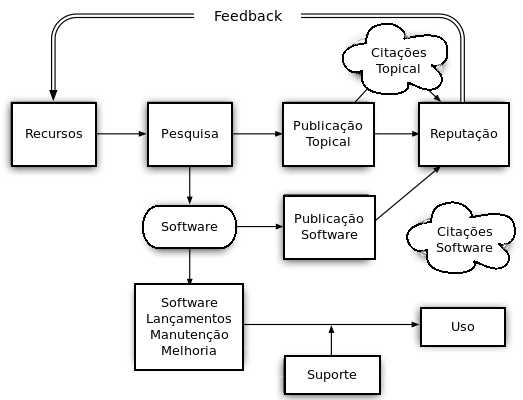
\includegraphics[scale=0.5]{imagens/scientific-reputation-diagram-dia.png}
  \caption{A depiction of the reputation incentives in a mixed science and software academic practice \cite{howison2011scientific}}
  \label{scientific-reputation-diagram}
\end{figure}

%ecossistema de software acadêmico está inserido num contexto de competição

Diferentemente de outras tecnologias, software pode ser copiado e distriduído
essencialmente sem custo, abrindo portas sem precedentes em nível para
compartilhamento e inovação colaborativa \cite{howison2011scientific}, no
entando, estar em algum ponto no contexto de competição da economia de
reputação científica, em alguns pontos, como no mecanismo de crédito acadêmico
às produções ser potencialmente problemático para a colaboração e manutenção
\cite{howison2011scientific}.

No entanto tem se percebido que o ecossistema de software acadêmico tem perdido
oportunidade de colaboração visto que estão inseridos neste contexto ....
competição, muitos softwares utilizados em pesquisas não são mencionados pelos
seus autores causando impacto negativo em sua visibilidade, reconhecimento e
consequentemente ...  \cite{howison2016software}. Esta reflexão tem mostrado,
por exemplo, que muitos estudos em engenharia de software sofrem de
dificuldades de repetição \cite{Tang2016}, e apontam problemas específicos
relacionados à manutenabilidade e a sustentabilidade técnica dos softwares
acadêmicos.

Este cenário, além de desacelerar o progresso geral da ciência gerando
retrabalho, faz surgir questionamentos sobre as conclusões dessas pesquisas,
especialmente quando grande parte dos pesquisadores não sabem o quão confiável
seus softwares são. Junto com estas questões estão as questões de como
influenciar o ecossistema, incluindo questões de pontos de inflexão que levam
ao uso coalescente, bem como a intervenções políticas diretas incentivando o
uso de componentes específicos.

%%%%%%%%%%%%%%%%%%%%%%%%%%%%%%%%%%%%%%%%%%%%%%%%%%%%%%%%%%%%%%

%While some of these seem relatively unproblematic, such as commercial
%production in fields with immediately valuable applications, others appear
%problematic. In particular we highlighted the potentially pernicious
%implications of the academic credit production system for collaboration and
%maintenance 

%Adicionalmente as relacões entre os atores do ecosistema como um todo
%são de mútuo interesse (mutualismo):

%O relacionamento entre os atores em um ecossistema de software, por outro lado,
%são caracterizados pela alto espectro de relacionamentos simbioticos.

%Dependendo dos atores e suas atividades, dois atores podem ter benefícios
%mútuos (mutualismo), estar em competição direta (competition/antagonism),
%estarem não afetados (neutralism) ou um não afetado enquanto o outro é
%beneficiado (amensalism) ou prejudicado (parasitism) por seu relacionamento

%Recursos são devotados para a produção de software acadêmico. Usuários finais
%cientistas (diretamente ou indiretamente) usam softwares acadêmicos para fazer
%ciência, resultando em impacto científico. 

%historia da citacao na ciencia, como isso promove o avanço, problemas para
%citacao em artefatos digitais, solucao para identificador unico de autores de
%artigos, orcid.org resolve este problema, o mesmo para identificar artefatos
%digitais é o doi.org

%em pesquisas sobre análise de código, ferramentas de analise estatica tem
%recebido significante mais atencao que outras tecnicas, tecnicas com formal e
%bem definidos processos recebem mais atencao de pesquisa e escrutinio porque
%estudos irao avaliar seu processo e elementos, entretanto, isto nao
%necessariamente significa que tecnica é melhor; The survey concluded that 1)
%the adoption of static code analysis techniques in the industry is influenced
%by the software life cycle model, while software product type and company size
%doesn’t have an influence. 2) The amount of attention a static code analysis
%technique has received in research doesn’t necessarily influence its adoption
%in industry indicating a gap between research and industry 3) company size,
%product type, and life cycle model do influence professionals perception on
%benefits/limitations.  \cite{ilyas2016static}

%A seção \ref{analise-estatica} apresenta uma definição geral da análise
%estática de código fonte, suas aplicações, sua anatomia, seus formatos de
%representação intermediária e técnicas mais comuns. 

%De acordo com \citeonline{Chess2007}, as atividades em que análise
%estática de código fonte é empregada, destacam-se:
%
%\begin{description}
%
%  \item \textit{Verificação de tipos}. 
%    A forma mais amplamente utilizada de análise estática, e uma das quais os
%    programadores estão mais familiarizados, é a checagem de tipo.
%    Previne que acidentalmente atribuam valores de forma incorreta a
%    variáveis. Ainda, ao capturar erros em tempo de compilação, esta checagem
%    de tipo previne erros em tempo de execução.
%
%  \item \textit{Verificação de estilo}. 
%    Os verificadores de estilo são um tipo de análise estática que aplicam regras
%    de forma mais superficial do que os verificadores de tipo. São regras
%    relacionadas a espaços em branco, nomes, funções depreciadas, comentários,
%    estrutura do programa, entre outros. Os erros reportados por verificadores de
%    estilo são aqueles que afetam a leitura e a manutenabilidade do
%    código fonte, não indicando potenciais erros em tempo de execução como
%    fariam os verificadores de tipo.
%
%  \item \textit{Compreensão de programas}. 
%    Ferramentas de compreensão de programa ajudam programadores a terem uma visão
%    clara frente a grandes programas de computador, ou seja, programas com
%    alto volume de código fonte. Ambientes de desenvolvimento integrados (IDE)
%    geralmente incluem funcionalidade de compreensão, por exemplo, ``encontrar
%    todos os usos de um certo método'' ou ``encontrar a declaração de uma
%    variável global''. Análises mais avançadas chegam a incluir, por exemplo,
%    refatoração automática. Estas ferramentas de compreensão também são úteis
%    para programadores interessados em entender código fonte escrito por
%    outros programadores.
%
%  \item \textit{Verificação de programas}.
%    Ferramentas de verificação de programa aceitam como entrada uma especificação
%    e um conjunto de código fonte e tenta provar que o código está deacordo
%    com a especificação. Quando a especificação é uma descrição completa de
%    todo o programa, a ferramenta de verificação poderá realizar uma checagem
%    de equivalência para garantir que o código fonte e a especificação
%    combinam de forma exata. Programadores raramente têm acesso a uma
%    especificação detalhada suficientemente para ser usada numa checagem de
%    equivalência, o trabalho de criar esta especificação pode ser maior do que
%    o trabalho de escrever o próprio código fonte do programa, desta forma
%    este tipo de verificação formal raramente acontece.
%
%  \item \textit{Localização de bugs}. 
%    Um localizador de bugs está
%    preocupado em apontar locais onde o programa, possivelmente, irá se
%    comportar de forma inesperada. A maioria das ferramentas de localização de
%    bugs são fáceis de usar porque costumam vir com um conjunto de regras
%    ({\it bug idioms}) para descrição de padrões de código que indicam bugs.
%    Algumas destas ferramentas costumam usar os mesmos algoritmos utilizados
%    por ferramentas de verificação de propriedade.
%
%  \item \textit{Avaliação de segurança}. 
%    Ferramentas de análise estática para segurança usam as mesmas técnicas
%    encontradas nas outras ferramentas, mas por ter um propósito diferente,
%    identificar problemas de segurança, aplicam estas técnicas de forma diferente.
%    As primeiras ferramentas de segurança (ITS4, RATS, Flawfinder) eram pouco mais
%    do que um {\it ``grep''} melhorado; na maior parte, elas escaneavam o código
%    procurando por funções como por exemplo {\it ``strcpy()''} que são
%    facilmente usadas de forma inadequada e devem ser inspecionadas
%    manualmente no processo de revisão de código fonte.
%
%\end{description}

%\subsection{Anatomia da análise de código fonte} \label{anatomia}
%
%Ferramentas de análise estática de código fonte estão organizadas em partes ou
%componentes, responsáveis por implementar três funções básicas: a) extração de dados, b) geração de representação
%intermediária, e c) análise \cite{Cruz2009, Binkley2007}.
%
%\begin{description}
%
%  \item \textit{Extração de dados}.
%    O processo de recuperar dados para futuro processamento ou armazenamento é
%    chamado de extração de dados. 
%
%    O primeiro componente da análise de código fonte é a extração de dados,
%    responsável por ler o código fonte do programa e gerar uma ou mais
%    representações intermediárias. Em essência, este componente converte a sintaxe
%    de um programa em uma outra sintaxe abstrata e mais adequada para análise
%    posterior.
%
%  \item \textit{Representação intermediária}.
%    Exportar os dados extraídos para uma representação intermediária é uma
%    estratégia comum para facilitar análise e transformação de dados e
%    possivelmente adição de metadados.
%
%    Os dados obtidos na extração precisam ser representados em um formato mais
%    abstrato. Esta é a responsabilidade do segundo componente da análise de
%    código fonte: armazenar os dados coletados usando uma representação
%    intermediária em formato mais adequado para análise automática, abstraindo
%    aspectos particulares do programa e da linguagem de programação.
%
%    Alguns tipos de representação intermediária têm sua origem na área de
%    compiladores, entre os formatos mais comuns, destacam-se:
%
%    \begin{multicols}{2}
%      \begin{itemize}
%        \item Árvore sintática abstrata
%        \item Grafo de fluxo de controle
%        \item Árvore sintática abstrata decorada
%        \item Grafo de dependência de módulos
%        \item Atribuição estática única
%        \item Grafo de dependência de valores
%      \end{itemize}
%    \end{multicols}
%
%    Estas representações podem ser utilizadas tanto na análise estática quanto
%    na análise dinâmica. O uso de um ou outro formato depende do tipo de
%    análise e seu propósito. Pode-se combinar diferentes tipos no sentido de
%    enriquecer e estruturar a informação extraída.
%
%  \item \textit{Análise}.
%    Este componente é responsável por realizar inferências a partir dos dados
%    representados internamente. O processo requer que as informações
%    armazenadas estejam interconectadas e também interrelacionadas com
%    conhecimento anterior. Esta análise pode gerar conhecimento quantitativo
%    ou qualitativo, como, por exemplo, métricas de software ou mineração de
%    dados, respectivamente. Técnicas de visualização podem ser usadas para
%    apoiar este processo.
%
%    Diversas técnicas foram desenvolvidas ao longo do tempo para realizar
%    análise, algumas delas são brevemente descritas na seção \ref{tecnicas}.
%
%\end{description}
%
%\subsection{Formatos de representação intermediária} \label{formatos}
%
%Essencialmente, um formato de representação intermediária é uma abstração precisa
%das propriedades de um programa representado em um domínio menor. Os
%compiladores normalmente constroem esta representação a fim de possuir um
%modelo do programa sendo compilado, é comum que compiladores utilizem diversos
%formatos durante o curso da compilação.
%
%Em ferramentas de análise estática estes formatos são utilizados durante a
%fase de análise para cumprir diversos objetivos, como por exemplo, calcular
%métricas de código fonte. A métrica de complexidade ciclomática de McCabe
%\cite{McCabe1976}, por exemplo, é definida com base no grafo de fluxo de controle ({\it Control Flow Graph - CFG}) do
%programa com o seguinte cálculo $CC = e - n + 2p$. Onde: {\bf e} é o número de
%arestas; {\bf n} é o número de nós; e {\bf p} é o número de componentes
%fortemente conectados no grafo.
%
%Assim, percebe-se que cada formato de representação intermediária pode ter fins
%e objetivos bastante distintos, dentre os formatos mais comuns podemos destacar
%\cite{Nielson2015, Stanier2013, Cruz2009, Ramalho1996}:
%
%\begin{description}
%
%  \item \textit{Árvore sintática abstrata}.
%    A árvore sintática abstrata (AST - {\it Abstract Syntax Tree}) representa um
%    programa tratando os elementos do código fonte como operadores e
%    operandos organizados em nós numa árvore, este formato de representação é
%    muito popular em tradutores {\it
%    source-to-source}\footnote{http://en.wikipedia.org/wiki/Source-to-source\_compiler}.
%
%  \item \textit{Grafo de fluxo de controle}.
%    O grafo de fluxo de controle (CFG - {\it Control Flow Graph} ou {\it Call Graph}) é um grafo direcionado
%    representando a estrutura de controle de um programa e sua sequência de
%    instruções, onde as arestas mostram os possíveis caminhos de execução. Este
%    formato é amplamente utilizado em métodos formais para otimização de
%    código fonte.
%
%  \item \textit{Grafo de fluxo de dados}.
%    O grafo de fluxo de dados (DFG - {\it Data Flow Graph}) é também um grafo
%    direcionado onde as arestas representam o fluxo de dados entre as
%    operações do programa, este formato pode ser visto como um companheiro do
%    grafo de fluxo de controle (CFG) e pode ser gerado ao longo de uma mesma
%    análise.
%
%  \item \textit{Árvore sintática abstrata decorada}.
%    Árvore sintática abstrata decorada (DAST - {\it Decorated Abstract Syntax Tree}) é
%    uma árvore sintática abstrata (AST) melhorada através de um processo de
%    definiçao de atributos para os símbolos do programa de forma declarativa
%    com uso de uma Gramática de
%    Atributos\footnote{https://en.wikipedia.org/wiki/Attribute\_grammar}.
%
%  \item \textit{Grafo de dependência de módulos}.
%    O grafo de dependência de módulos (MDG - {\it Module Dependence Graph}) é um grafo
%    onde os módulos são representados como nós e as arestas representam as
%    relacões entre eles, indicando dependência entre os mesmos.
%
%  \item \textit{Atribuição estática única}.
%    Atribuição estática única (SSA - {\it Static Single Assignment}) pode ser vista
%    como uma variação ou uma propriedade de outros formatos de representação
%    intermediária, é um método que faz cada variável ser atribuída apenas uma única
%    vez, facilitando a descoberta de informaçoes sobre os dados representados.
%
%  \item \textit{Grafo de dependência de valores}.
%    O grafo de dependência de valores (VDG - {\it Value Dependence Graph}) é uma
%    variação que melhora (ao menos para algumas análises) os resultados
%    obtidos a partir da atribuição estática única (SSA). Ele representa tanto
%    o fluxo de controle quanto o fluxo de dados e assim simplifica a análise.
%
%\end{description}
%
%\subsection{Técnicas de análise} \label{tecnicas}
%
%Inúmeras técnicas e métodos distintos podem ser utilizados pelas ferramentas
%de análise estática, seja com o objetivo de verificação de tipos, localização
%de bugs, compreensão de programas, avaliação de segurança, ou outra finalidade
%qualquer. Segundo \citeonline{German2003, Li2010, Hofer2010} as técnicas e
%métodos mais comumente encontrados nas ferramentas atuais são:
%
%\begin{description}
%
%  \item \textit{Análise léxica}.
%    A análise léxica é responsável por quebrar o programa em pequenos fragmentos
%    (ou {\it tokens}) e verificar se estes fragmentos são palavras válidas
%    para uma dada linguagem. A análise léxica não leva em consideração a
%    sintaxe do programa, sua semântica ou a interação entre módulos.
%
%  \item \textit{Combinação de padrões de texto}.
%    A combinação de padrões de texto ({\it Text-based Pattern Matching}) é a
%    maneira mais simples e rápida de procurar vulnerabilidades num código
%    fonte.
%
%  \item \textit{Inferência de tipos}.
%    A inferência de tipos ({\it Type inference}) refere-se a identificar o
%    tipo de variáveis e funções e avaliar se o acesso a elas está em
%    conformidade com as regras da linguagem. Linguagens de programação com
%    sistema de tipagem incluem mecanismos deste tipo de análise.
%
%  \item \textit{Análise de fluxo de dados}.
%    A análise de fluxo de dados ({\it Data flow analysis}) resume-se a coletar
%    informação semântica do código fonte do programa, e com métodos algébricos
%    deduzir a definição e uso das variáveis em tempo de compilação. O objetivo
%    é mostrar que nenhum caminho de execução do programa acessa uma variável
%    sem definição ou atribuição prévia.
%
%  \item \textit{Verificação de regra}.
%    A verificação de regra ({\it Rule checking}) consiste em checar a segurança
%    do programa através de um conjunto de regras pré-estabelecidas.
%
%  \item \textit{Análise de restrição}.
%    A análise de restrição ({\it Constraint analysis}) consiste em gerar
%    e resolver restrições no processo de análise de um programa.
%
%  \item \textit{Comparação caminho}.
%    Comparação caminho ({\it Patch comparison}) inclui comparação de caminho de
%    código fonte e de código-binário e é usada principalmente para encontrar
%    brechas de vulnerabilidade já ``conhecidas'' e previamente divulgadas por
%    fornecedores e praticantes da indústria de software.
%
%  \item \textit{Execução simbólica}.
%    A execução simbólica ({\it Symbolic execution}) é usada para representar
%    as entradas de um programa através do uso de valores simbólicos ao invés
%    de dados reais, produz expressões algébricas sobre a entrada dos símbolos
%    do programa durante o processo de implementação e pode detectar
%    possibilidade de erros.
%
%  \item \textit{Interpretação abstrata}.
%    Interpretação abstrata ({\it Abstract interpretation}) é uma descrição
%    formal da análise do programa. Pelo fato de apenas controlar atributos de
%    programa de preocupaçao dos usuários, a interpretação da análise semântica
%    é similar ao seu significado semântico real.
%
%  \item \textit{Prova de teoremas}.
%    Prova de teoremas ({\it Theorem proving}) é baseada na análise semântica do
%    programa. Converte o programa em fórmulas lógicas e então tenta provar que
%    o programa é um teorema válido usando regras e axiomas.
%
%  \item \textit{Verificação de modelo}.
%    O processo de verificação de modelos ({\it Model checking}) primeiro constrói
%    um modelo formal do programa tal como uma máquina de estados ou um grafo
%    direcionado, então examina e compara o modelo para verificar se o sistema
%    cumpre as características pré-definidas. Esta técnica requer a definição e
%    descrição das propriedades que devem ser verificados por um pedaço de
%    software.
%
%  \item \textit{Verificação formal}.
%    Verificação formal ({\it Formal Checking} ou {\it Compliance Analysis}) é o
%    processo de provar de forma automatizada que o código do programa está
%    correto em relação a uma especificação formal dos seus requisitos.
%
%  \item \textit{Análise de fluxo da informação}.
%    Análise de fluxo da informação ({\it Information Flow Analysis}) identifica
%    como a execução de uma unidade de código cria dependência entre entradas e
%    saídas.
%
%  \item \textit{Verificação de sintaxe}.
%    Verificação de sintaxe ({\it Syntax Checks}) tem o objetivo de encontrar
%    violação de regras tais como expressões mal-formadas ou fora do padrão.
%
%  \item \textit{Verificação de intervalo}.
%    A análise de verificação de intervalo ({\it Range Checking}) tem o objetivo
%    de verificar que os valores dos dados permanecem dentro de intervalos
%    especificados, bem como manter a precisão especificada.
%
%\end{description}

